\documentclass[border=6pt]{standalone}
\usepackage{tikz}
\usepackage{sfmath}
\renewcommand{\familydefault}{\sfdefault}
\usetikzlibrary{arrows.meta,positioning,decorations.pathreplacing,fit,backgrounds,calc,shapes.geometric}
\definecolor{cExtract}{HTML}{2C6FB0}
\definecolor{cExtractL}{HTML}{DCE8F5}
\definecolor{cReduce}{HTML}{C77400}
\definecolor{cReduceL}{HTML}{FBE8CC}
\definecolor{cClass}{HTML}{2E7D5B}
\definecolor{cClassL}{HTML}{D8ECE2}
\definecolor{cOut}{HTML}{4A4A8A}
\definecolor{cInk}{HTML}{222222}
\tikzset{
  font=\sffamily,
  hdr/.style={rounded corners=3pt, draw=none, text=white, font=\sffamily\bfseries\small, inner sep=5pt, align=center, minimum height=8mm},
  card/.style={rounded corners=3pt, draw=#1, line width=0.8pt, fill=white, align=center, inner sep=4pt, font=\small},
  item/.style={rounded corners=2pt, draw=#1!70, fill=#1!8, align=center, font=\footnotesize, minimum width=24mm, minimum height=6mm, inner sep=2pt},
  flow/.style={-{Stealth[length=2.5mm]}, line width=0.9pt, draw=cInk},
  outb/.style={rounded corners=3pt, fill=cOut, text=white, font=\sffamily\bfseries\small, align=center, inner sep=5pt, minimum height=9mm},
}
\tikzset{
  img/.style={rounded corners=2pt, draw=cInk!60, fill=gray!12, align=center, font=\footnotesize, minimum width=14mm, minimum height=11mm, inner sep=2pt},
  proc/.style={rounded corners=3pt, draw=cExtract, line width=0.9pt, fill=cExtractL, align=center, font=\small, minimum height=9mm, inner sep=4pt},
  vecg/.style={rounded corners=3pt, draw=cClass, line width=0.9pt, fill=cClassL, align=center, font=\footnotesize, minimum height=8mm, inner sep=3pt},
  vecy/.style={rounded corners=3pt, draw=cReduce, line width=0.9pt, fill=cReduceL, align=center, font=\footnotesize, minimum height=8mm, inner sep=3pt},
  redb/.style={rounded corners=3pt, draw=cReduce, line width=0.9pt, fill=white, align=center, font=\small, minimum height=9mm, inner sep=4pt},
  clf/.style={rounded corners=3pt, draw=cClass, line width=0.9pt, fill=cClassL, align=center, font=\small, minimum height=9mm, inner sep=4pt},
  res/.style={rounded corners=3pt, fill=cOut, text=white, font=\sffamily\bfseries\footnotesize, align=center, minimum height=9mm, inner sep=4pt},
}
\tikzset{
  vstep/.style={rounded corners=3pt, line width=0.8pt, align=center, font=\footnotesize, minimum width=34mm, minimum height=8mm, inner sep=3pt},
  vflow/.style={-{Stealth[length=2mm]}, line width=0.8pt, draw=cInk},
}
\tikzset{
  vb/.style={rounded corners=3pt, line width=0.8pt, align=center, font=\scriptsize, minimum width=22mm, minimum height=7mm, inner sep=2pt},
  vw/.style={rounded corners=3pt, line width=0.8pt, align=center, font=\footnotesize, minimum width=46mm, minimum height=8mm, inner sep=3pt},
}
\newcommand{\mergeinto}[2]{% #1 = lista de nós origem (csv), #2 = nó destino
  \coordinate (by) at ([yshift=4mm]#2.north);
  \foreach \s in {#1}{\draw[line width=0.8pt,draw=cInk] (\s.south) -- (\s.south|-by);}
}

\begin{document}
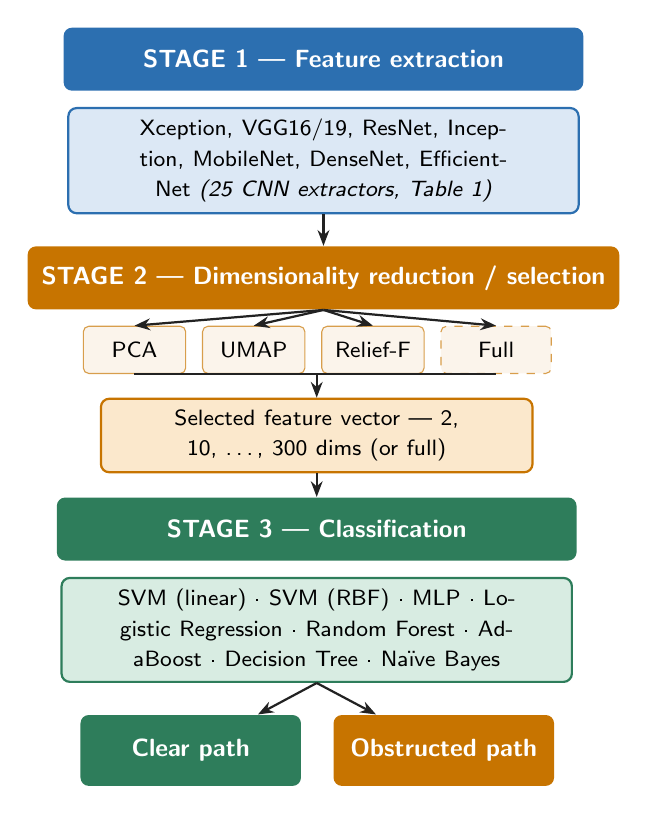
\begin{tikzpicture}[node distance=4.5mm]
\node[hdr, fill=cExtract, minimum width=66mm] (h1){STAGE 1 — Feature extraction};
\node[card=cExtract, below=2mm of h1, text width=62mm, fill=cExtractL] (cnn)
  {\footnotesize Xception, VGG16/19, ResNet, Inception, MobileNet, DenseNet, EfficientNet \textit{(25 CNN extractors, Table 1)}};
\node[hdr, fill=cReduce, minimum width=66mm, below=4mm of cnn] (h2){STAGE 2 — Dimensionality reduction / selection};
\node[item=cReduce, below=2mm of h2.south, xshift=-24mm, minimum width=13mm] (pca){PCA};
\node[item=cReduce, right=2mm of pca, minimum width=13mm] (umap){UMAP};
\node[item=cReduce, right=2mm of umap, minimum width=13mm] (rel){Relief-F};
\node[item=cReduce, right=2mm of rel, minimum width=14mm, draw=cReduce!70, dashed] (full){Full};
\node[card=cReduce, below=3mm of umap, xshift=8mm, text width=52mm, fill=cReduceL] (fv){\footnotesize Selected feature vector — 2, 10, \ldots, 300 dims (or full)};
\node[hdr, fill=cClass, minimum width=66mm, below=3mm of fv] (h3){STAGE 3 — Classification};
\node[card=cClass, below=2mm of h3, text width=62mm, fill=cClassL] (clf)
  {\footnotesize SVM (linear) · SVM (RBF) · MLP · Logistic Regression · Random Forest · AdaBoost · Decision Tree · Na\"ive Bayes};
\node[outb, fill=cClass, below=4mm of clf, xshift=-16mm, minimum width=28mm] (o1){Clear path};
\node[outb, fill=cReduce, right=4mm of o1, minimum width=28mm] (o2){Obstructed path};
\draw[vflow](cnn)--(h2); 
\foreach \x in {pca,umap,rel,full} \draw[vflow](h2.south)-- (\x.north);
\coordinate (by) at ([yshift=3mm]fv.north);
\foreach \x in {pca,umap,rel,full}{\draw[line width=0.8pt,draw=cInk] (\x.south) -- (\x.south|-by);}
\draw[line width=0.8pt,draw=cInk] (pca.south|-by) -- (full.south|-by);
\draw[vflow] (fv.north|-by) -- (fv.north);
\draw[vflow](fv)--(h3); \draw[vflow](clf.south)--(o1); \draw[vflow](clf.south)--(o2);
\end{tikzpicture}
\end{document}
